\documentclass[12pt,twoside, a4paper, twocolumn]{article}
\usepackage[utf8]{inputenc}
\usepackage[brazil]{babel}
\usepackage[margin = 0.5in]{geometry}
\usepackage{amsmath}
\usepackage{amsthm}
\usepackage{amssymb}
\usepackage{amsthm}
\usepackage{setspace}
\usepackage[americanvoltages,fulldiodes,siunitx]{circuitikz}
\usepackage{lipsum}
\usepackage{pgfplots}
\usepackage{ifthen}
\usepackage{adjustbox}
\usepackage[section]{placeins}
\usepackage{hyperref}
\usepackage{graphicx}
\usepackage{amsmath}
\usepackage{amsthm}
\usepackage{amssymb}
\usepackage{amsthm}
\usepackage{setspace}
\usepackage[americanvoltages,fulldiodes,siunitx]{circuitikz}
\usepackage{lipsum}
\usepackage{pgfplots}
\usepackage{ifthen}
\usepackage{adjustbox}
\usepackage[section]{placeins}
\usepackage{hyperref}
\usepackage{graphicx}
\usepackage{adjustbox}
 
\pgfplotsset{compat=newest}
 
\graphicspath{ {./images/} }
 
%  #1 color - optional #2 x_0 #3 y_0 #4 x_f #5 y_f #6 name - optional  #7 true if adding lines to axis
 
\newcommand{\drawvector} [9] [color=cyan] {
   \draw[line width=1.5pt,#1,-stealth](axis cs: #2, #3)--(axis cs: #4, #5) node[anchor=south west]{$#6$};
 
  
 
\ifthenelse{\equal{#7}{true}}{
   \draw[line width=1pt,#1, dashed](axis cs: #4, #5)--(axis cs: #4, 0) node[anchor= north west]{$#8$};
   \draw[line width=1pt,#1, dashed](axis cs: #4, #5)--(axis cs: 0, #5) node[anchor=south east]{$#9$};
   }
   {}
}
 
\newcommand\deriv[2]{\frac{\mathrm d #1}{\mathrm d #2}}
 
 
\title{Terceiro Relatório de Lab de Circuitos}
\author{Henrique da Silva \\ hpsilva@proton.me}
\date{\today}
\pgfplotsset{width = 10cm, compat = 1.9}
 
 
\begin{document}
\maketitle
\pagenumbering{gobble}
\newpage
%pagenumbering{roman}
\tableofcontents
\newpage



\section{Introdução}


\subparagraph*{Neste relatório, vamos discutir amplificadores operacionais, e como controlar uma saída de corrente a partir de duas correntes de entrada.}

\subparagraph*{Todos arquivos utilizados para criar este relatorio, e o relatorio em si estão em:  \url{https://github.com/Shapis/ufpe_ee/tree/main/4th semester/lab circuitos}}




\subsection{O Amp Op}
\subparagraph*{}
\begin{center}
    \begin{circuitikz}
        \draw (0,2)
        node[ocirc,  label=180:$V_{1}$]{};
        \draw (2.5,0)
        node[ocirc,  label=90:$V_{a}$]{};
        \draw (0,0)
        node[ocirc,  label=180:$V_{2}$]{};
        \draw (6,-0.5)
        node[ocirc,  label=2:$V_{0}$]{};
        \draw (0,2) to[resistor=$R_1$] (2,2) -- (2,0) to[resistor=$R_2$] (0,0);
        \draw (2,0) -- (3,0) -- (3,2) to[resistor=$R_3$] (5,2) -- (5,-0.5) -- (6,-0.5);
        \draw (2,-1) node[above]{$v_i$} to[short, o-] ++(1,0)
        node[op amp, noinv input down, anchor=+](OA){\texttt{}}
        ;
        \draw (2,-1) -- (2,-1.5);
        \draw (2,-1.5)
        node[rground]{};

    \end{circuitikz}
\end{center}

\subparagraph*{Neste caso o amp op faria uma multiplicação da corrente $V_a$ na saída $V_0$ de acordo com um fator de multiplicação $A$}





\section{Analise nodal do circuito}


\subparagraph*{Primeiro vale lembrar que a resistência de Thevenin e a de Norton são iguais. Logo obtendo uma também obteremos a outra.
}

\subparagraph*{Neste caso, resolvendo o sistema vamos obter que esta resistência é igual a $R_{c}$}

\begin{equation}
    \begin{aligned}
         & \frac{V_a - V_1}{R_1} + \frac{V_a-V_0}{R_3} + \frac{V_a-V_2}{R_2} = 0 \\
         & V_0 = -A*V_a
    \end{aligned}
\end{equation}

\subparagraph*{Que nos da:}

\begin{equation}
    V_0 = -\frac{A R_1 R_3 V_2 + A R_2 R_3 V_1}{(R_2 + R_1)R_3 + (A + 1) R_1 R_2}
\end{equation}

\subparagraph*{E para o caso específico do amp op ideal, fazemos $A$ tender a infinito e simplesmente temos:}

\begin{equation}
    \begin{aligned}
        V_0 & = -\frac{R_1 R_3 V_2 + R_2 R_3 V_1}{R_1 R_2} \\
        V_0 & = - \frac{R_3}{R_1}V_1 - \frac{R_3}{R_2}V_2  \\
    \end{aligned}
\end{equation}

\subparagraph*{Daí podemos juntar (1) com (3) e obter:}

\begin{equation}
    \begin{aligned}
        A_{v_1} & = -\frac{R_3}{R_1} \\
        A_{v_2} & = -\frac{R_3}{R_2} \\
    \end{aligned}
\end{equation}


\subparagraph*{Também é importante notar que as resistências vistas de $V_1$ e $V_2$ são as seguintes:}
\begin{equation}
    I_n = \frac{V_1-V_a}{R_n} \rightarrow R_{im_n} = \frac
    {V_n}{I_n} = R_n * \frac{V_n}{V_n - V_a} = R_n
\end{equation}

\section{Resultados preliminares}

\subparagraph*{Aqui vamos fazer uma análise utilizando a teoria demonstrada acima para saber como montar o circuito para termos um ganho $A_1 = -2$ e $A_2 = -4$}
\subsection{Montando o circuito}
\subparagraph*{Nos termos da equação (4) como os ganhos se comportam a partir das resistências do circuito. Então, basta resolvermos este sistema utilizando valores de resistores comerciais.}



\begin{equation}
    \begin{aligned}
        A_{v_1} & = -\frac{R_3}{R_1} = -2 \\
        A_{v_2} & = -\frac{R_3}{R_2} = -4 \\
    \end{aligned}
\end{equation}

\subparagraph*{Podemos então escolher resistores com aproximadamente os seguintes valores:}

\begin{equation}
    \begin{aligned}
        R_1 & \approx 100k \varOmega \\
        R_2 & \approx 47k \varOmega  \\
        R_3 & \approx 220k \varOmega \\
    \end{aligned}
\end{equation}

\subsection{Valores esperados}

\subparagraph*{Vamos analisar as seguintes combinações de tensões em $V_1$ e $V_2$: ${-1,2 ; -0,6 ; 0 ; 0,6 ; 1,2}$}

\subparagraph*{A análise será feita em $C\#$ e esta em: \url{https://github.com/Shapis/ufpe_ee/blob/main/4th semester/lab circuitos/Relatorio 3/Program.cs}}

\begin{center}
    \begin{tabular}{ |c|ccccc| }
        \hline
        $V_2 \downarrow / V_1 \rightarrow $ & $-1.2V$ & $-0.6V$ & $0.0V$  & $0.6V$  & $1.2V$  \\
        $-1.2V$                             & $8.26$  & $6.94$  & $5.62$  & $4.30$  & $2.98$  \\
        $ -0.6V$                            & $5.45$  & $4.13$  & $2.81$  & $1.49$  & $0.17$  \\
        $0.0V$                              & $2.64$  & $1.32$  & $0$     & $-1.32$ & $-2.64$ \\
        $ 0.6V$                             & $-0.17$ & $-1.49$ & $-2.81$ & $-4.13$ & $-5.45$ \\
        $ 1.2V$                             & $-2.98$ & $-4.30$ & $-5.62$ & $-6.94$ & $-8.26$ \\
        \hline
    \end{tabular}
\end{center}

\section{Medicoes no laboratorio}

\subparagraph*{Nesta etapa nós montamos o circuito como indicado na secao 1.1, com única diferença que nós alimentamos o Amp Op com uma diferença de potencial de $20V$ já que ele é um elemento ativo.}

\subparagraph*{Foto do circuito abaixo:}
\subparagraph*{}

\begin{adjustbox}{scale=0.3}
    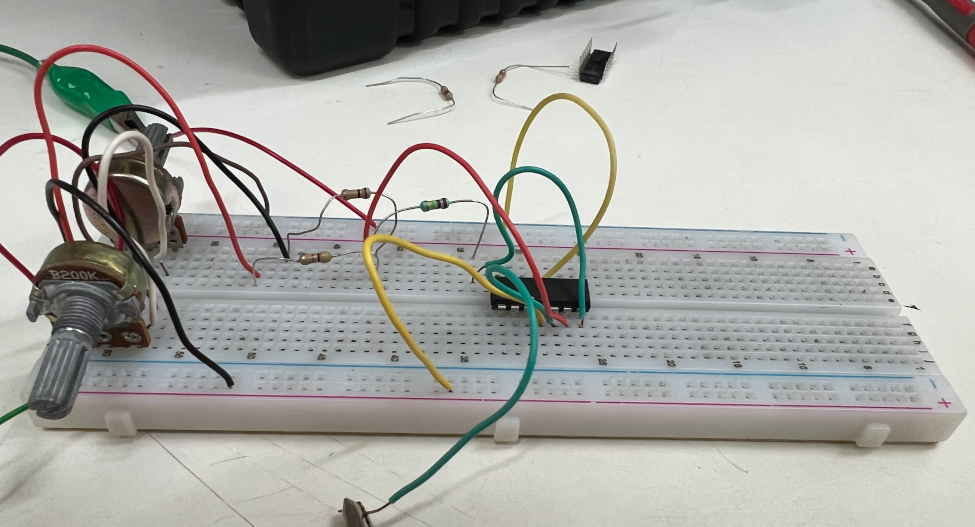
\includegraphics{circuito.png}
\end{adjustbox}

\subsection{Valores experimentais}

\begin{center}
    \begin{tabular}{ |c|ccccc| }
        \hline
        $V_2 \downarrow / V_1 \rightarrow $ & $-1.2V$ & $-0.6V$ & $0.0V$  & $0.6V$  & $1.2V$  \\
        $-1.2V$                             & $8.37$  & $7.03$  & $5.72$  & $4.31$  & $3.01$  \\
        $ -0.6V$                            & $5.48$  & $4.18$  & $2.85$  & $1.45$  & $0.23$  \\
        $0.0V$                              & $2.67$  & $1.36$  & $0.04$  & $-1.31$ & $-2.62$ \\
        $ 0.6V$                             & $-0.21$ & $-1.54$ & $-2.84$ & $-4.18$ & $-5.53$ \\
        $ 1.2V$                             & $-3.03$ & $-4.36$ & $-5.67$ & $-7$    & $-8.32$ \\
        \hline
    \end{tabular}
\end{center}

\subparagraph*{Resolvendo este sistema linear da seguinte maneira:}

\begin{equation}
    V_1^n A_1^n + V_2^n A_2^n = V_0^n \\
\end{equation}


\subparagraph*{Temos que o ganho $A_1$ real é $-2.2$ e o ganho $A_2$ real é $-4.7$}

\subparagraph*{Pelo método dos mínimos quadrados. O que fiz foi o seguinte: Fixei o $V_2$ em um valor específico, e variei o $V_1$ para cada valor $V_0$ obtido.}

\subparagraph*{Isto me deu cinco retas aproximadas pelo método dos mínimos quadrados.}

\subparagraph*{Com as cinco equações em mãos fiz o mesmo passo que utilizei para conseguir o ganho real não aproximado por este método de $A_1$ e $A_2$ e obtive os mesmos ganhos que havia obtido anteriormente. $A_1 = -4.7$ e $A_2 -2.2$}



\section{Conclusões}

\subparagraph*{Nesta prática vimos como controlar o de tensão em um circuito a partir de uma montagem simples de resistores e um amplificador operacional.}

\subparagraph*{Também aprendemos a utilizar potenciômetros para o controle de tensões de entrada em um circuito.}

\end{document}